\chapter{Géométrie dans l'espace}

Ce chapitre transpose les outils vectoriels et analytiques de la géométrie plane à l'espace à trois dimensions. Nous allons étudier les droites, les plans, le produit scalaire dans l'espace, et caractériser les plans par leurs équations cartésiennes.

\section{Vecteurs, Droites et Plans dans l'Espace}

\subsection{Représentation paramétrique d'une droite}

Une droite dans l'espace est entièrement déterminée par un point et un vecteur directeur.

\begin{definition}[Représentation paramétrique d'une droite]
Soit $D$ la droite passant par le point $A(x_0, y_0, z_0)$ et de vecteur directeur $\vec{u}(a, b, c)$.
Un point $M(x, y, z)$ appartient à $D$ si et seulement s'il existe un réel $t$ (le paramètre) tel que $\vec{AM} = t \vec{u}$.
Le système d'équations suivant est appelé **représentation paramétrique de la droite $D$** :
\[
\begin{cases}
x = x_0 + a t \\
y = y_0 + b t \\
z = z_0 + c t
\end{cases} \quad (t \in \R)
\]
\end{definition}

\subsection{Vecteurs coplanaires et définition d'un plan}

\begin{definition}[Vecteurs coplanaires]
Trois vecteurs sont dits **coplanaires** si leurs représentants ayant une même origine ont leurs extrémités dans un même plan.
\end{definition}

\begin{definition}[Représentation d'un plan]
Un plan $\mathcal{P}$ est déterminé par un point $A$ et deux vecteurs $\vec{u}$ et $\vec{v}$ **non colinéaires** (appelés vecteurs directeurs du plan).
Un point $M$ appartient à $\mathcal{P}$ si et seulement s'il existe deux réels $t$ et $s$ tels que :
\[
\vec{AM} = t \vec{u} + s \vec{v}
\]
\end{definition}

\section{Produit Scalaire et Orthogonalité dans l'Espace}

Dans toute la suite, l'espace est muni d'un repère orthonormé $(O; \vec{\imath}, \vec{\jmath}, \vec{k})$.

\subsection{Expression analytique du produit scalaire}

\begin{definition}[Produit scalaire]
Soient $\vec{u}(x, y, z)$ et $\vec{v}(x', y', z')$ deux vecteurs de l'espace. Le produit scalaire $\vec{u} \cdot \vec{v}$ est le nombre réel défini par :
\[
\vec{u} \cdot \vec{v} = x x' + y y' + z z'
\]
La norme du vecteur $\vec{u}$ est $\|\vec{u}\| = \sqrt{x^2+y^2+z^2}$, et la distance entre $A(x_A, y_A, z_A)$ et $B(x_B, y_B, z_B)$ est :
\[
AB = \sqrt{(x_B-x_A)^2 + (y_B-y_A)^2 + (z_B-z_A)^2}
\]
\end{definition}

\subsection{Orthogonalité}

\begin{definition}[Orthogonalité d'une droite et d'un plan]
Une droite $D$ est orthogonale à un plan $\mathcal{P}$ si elle est orthogonale à deux droites sécantes de $\mathcal{P}$.
Elle est alors orthogonale à toutes les droites du plan $\mathcal{P}$.
\end{definition}

\section{Équation Cartésienne d'un Plan}

\subsection{Vecteur normal à un plan}

\begin{definition}[Vecteur normal]
On dit qu'un vecteur non nul $\vec{n}$ est un **vecteur normal** au plan $\mathcal{P}$ si la droite dirigée par $\vec{n}$ est orthogonale au plan $\mathcal{P}$. Le vecteur $\vec{n}$ est alors orthogonal à tout vecteur directeur du plan $\mathcal{P}$.
\end{definition}

\begin{center}
\begin{tikzpicture}[scale=1.2]
  % Le plan P dessiné comme un parallélogramme
  \draw[fill=defbg!50, draw=defcolor, thick] (0,0) -- (4,0.5) -- (5,2.5) -- (1,2) -- cycle;
  \node[above left] at (4.5, 2.3) {$\mathcal{P}$};
  
  % Point A dans le plan
  \coordinate (A) at (2.5, 1.25);
  \fill[black] (A) circle (1.5pt) node[below] {$A$};
  
  % Vecteurs directeurs u et v
  \draw[->, >=latex, color=thcolor, very thick] (A) -- (3.7, 1.4) node[above] {$\vec{u}$};
  \draw[->, >=latex, color=thcolor, very thick] (A) -- (1.6, 1.8) node[above] {$\vec{v}$};
  
  % Vecteur normal n
  \draw[->, >=latex, color=methcolor, very thick] (A) -- (2.5, 3.25) node[right] {$\vec{n}$};
  
  % Symboles d'angle droit en 3D
  \draw[gray, thin] (2.5, 1.55) -- (2.7, 1.575) -- (2.7, 1.275);
  \draw[gray, thin] (2.5, 1.5) -- (2.3, 1.55) -- (2.3, 1.3);
\end{tikzpicture}
\end{center}

\subsection{Équation cartésienne}

\begin{theoreme}[Équation cartésienne d'un plan]
\begin{itemize}
    \item Tout plan $\mathcal{P}$ admettant un vecteur normal $\vec{n}(a, b, c)$ possède une équation cartésienne de la forme :
    \[
    a x + b y + c z + d = 0
    \]
    où $d$ est un réel.
    \item Réciproquement, pour tous réels $a$, $b$, $c$ non tous nuls, l'ensemble des points $M(x, y, z)$ tels que $ax+by+cz+d=0$ est un plan de vecteur normal $\vec{n}(a, b, c)$.
\end{itemize}
\end{theoreme}

\section{Le Produit Vectoriel et Applications}

Le produit vectoriel est une opération propre à l'espace tridimensionnel qui associe à deux vecteurs un troisième vecteur orthogonal aux deux premiers.

\subsection{Définition et expression analytique}

Dans l'espace muni d'un repère orthonormé direct $(O; \vec{\imath}, \vec{\jmath}, \vec{k})$ :

\begin{definition}[Produit vectoriel]
Soient $\vec{u}(x, y, z)$ et $\vec{v}(x', y', z')$ deux vecteurs de l'espace.
On appelle \textbf{produit vectoriel} de $\vec{u}$ et $\vec{v}$, noté $\vec{u} \wedge \vec{v}$ (ou $\vec{u} \times \vec{v}$), le vecteur dont les coordonnées sont définies par :
\[
\vec{u} \wedge \vec{v} = \begin{pmatrix} y z' - z y' \\ z x' - x z' \\ x y' - y x' \end{pmatrix}
\]
\end{definition}

\begin{propriete}[Propriétés géométriques]
Soient deux vecteurs non colinéaires $\vec{u}$ et $\vec{v}$. Le vecteur $\vec{w} = \vec{u} \wedge \vec{v}$ possède les caractéristiques suivantes :
\begin{itemize}
    \item \textbf{Direction} : Le vecteur $\vec{w}$ est orthogonal à la fois à $\vec{u}$ et à $\vec{v}$. Il est donc normal au plan dirigé par $\vec{u}$ et $\vec{v}$.
    \item \textbf{Sens} : Le trièdre $(\vec{u}, \vec{v}, \vec{w})$ est direct (règle des trois doigts de la main droite).
    \item \textbf{Norme} : La norme de $\vec{w}$ est donnée par :
    \[
    \|\vec{u} \wedge \vec{v}\| = \|\vec{u}\| \times \|\vec{v}\| \times \sin(\theta)
    \]
    où $\theta \in [0, \pi]$ désigne l'angle entre les vecteurs $\vec{u}$ et $\vec{v}$.
\end{itemize}
\end{propriete}

\begin{propriete}[Propriétés algébriques]
Pour tous vecteurs $\vec{u}$, $\vec{v}$, $\vec{w}$ et pour tout réel $\lambda$ :
\begin{itemize}
    \item \textbf{Anti-symétrie} : $\vec{u} \wedge \vec{v} = - (\vec{v} \wedge \vec{u})$.
    \item \textbf{Bilinérarité} : 
    \[
    \vec{u} \wedge (\vec{v} + \vec{w}) = \vec{u} \wedge \vec{v} + \vec{u} \wedge \vec{w}
    \]
    \[
    (\lambda \vec{u}) \wedge \vec{v} = \lambda (\vec{u} \wedge \vec{v})
    \]
    \item \textbf{Condition de colinéarité} : $\vec{u} \wedge \vec{v} = \vec{0} \iff \vec{u}$ et $\vec{v}$ sont colinéaires.
\end{itemize}
\end{propriete}

\subsection{Applications géométriques}

\subsubsection{1. Aire d'un triangle et d'un parallélogramme}
\begin{itemize}
    \item \textbf{Aire d'un triangle} : L'aire du triangle $ABC$ dans l'espace est égale à :
    \[
    \mathcal{A}(ABC) = \frac{1}{2} \|\vec{AB} \wedge \vec{AC}\|
    \]
    \item \textbf{Aire d'un parallélogramme} : L'aire du parallélogramme $ABCD$ de vecteurs directeurs $\vec{AB}$ et $\vec{AD}$ est égale à :
    \[
    \mathcal{A}(ABCD) = \|\vec{AB} \wedge \vec{AD}\|
    \]
\end{itemize}

\subsubsection{2. Distance d'un point à une droite dans l'espace}
Soit une droite $D(A, \vec{u})$ passant par le point $A$ et de vecteur directeur $\vec{u}$, et soit $M$ un point quelconque de l'espace.
La distance du point $M$ à la droite $D$ est donnée par la formule :
\[
d(M, D) = \frac{\|\vec{AM} \wedge \vec{u}\|}{\|\vec{u}\|}
\]

\section{Équation de la Sphère et Intersections}

La sphère est l'ensemble des points de l'espace situés à une même distance (le rayon) d'un point donné (le centre). L'étude analytique de la sphère et de ses intersections avec des droites et des plans est une composante essentielle de la géométrie analytique de l'espace.

\subsection{Équation cartésienne d'une sphère}

\begin{theoreme}[Équation d'une sphère définie par son centre et son rayon]
Soit $\Omega(x_0, y_0, z_0)$ un point de l'espace et $R$ un réel strictement positif.
La sphère $\mathcal{S}$ de centre $\Omega$ et de rayon $R$ est l'ensemble des points $M(x, y, z)$ de l'espace vérifiant :
\[
(x - x_0)^2 + (y - y_0)^2 + (z - z_0)^2 = R^2
\]
Cette équation est appelée \textbf{l'équation cartésienne de la sphère} $\mathcal{S}$.
\end{theoreme}

\begin{theoreme}[Sphère définie par son diamètre]
Soient $A(x_A, y_A, z_A)$ et $B(x_B, y_B, z_B)$ deux points distincts de l'espace.
La sphère $\mathcal{S}$ de diamètre $[AB]$ est l'ensemble des points $M(x, y, z)$ de l'espace vérifiant la condition d'orthogonalité :
\[
\vec{MA} \cdot \vec{MB} = 0 \iff (x - x_A)(x - x_B) + (y - y_A)(y - y_B) + (z - z_A)(z - z_B) = 0
\]
Le centre $\Omega$ de la sphère est le milieu du segment $[AB]$ et son rayon vaut $R = \frac{AB}{2}$.
\end{theoreme}

\begin{propriete}[Détermination géométrique de l'ensemble $x^2 + y^2 + z^2 - 2ax - 2by - 2cz + d = 0$]
Soient $a, b, c$ et $d$ quatre réels. Soit $(E)$ l'ensemble des points $M(x, y, z)$ vérifiant l'équation :
\[
x^2 + y^2 + z^2 - 2ax - 2by - 2cz + d = 0
\]
En utilisant la forme canonique, cette équation s'écrit :
\[
(x - a)^2 + (y - b)^2 + (z - c)^2 = a^2 + b^2 + c^2 - d
\]
Soit $H = a^2 + b^2 + c^2 - d$. On a trois cas :
\begin{itemize}
    \item Si $H > 0$, alors $(E)$ est la sphère de centre $\Omega(a, b, c)$ et de rayon $R = \sqrt{H}$.
    \item Si $H = 0$, alors $(E)$ est réduit au seul point $\Omega(a, b, c)$.
    \item Si $H < 0$, alors $(E)$ est l'ensemble vide ($\emptyset$).
\end{itemize}
\end{propriete}

\subsection{Intersection d'une sphère et d'un plan}

Soit $\mathcal{S}$ une sphère de centre $\Omega$ et de rayon $R$, et $\mathcal{P}$ un plan. Soit $d = d(\Omega, \mathcal{P})$ la distance du centre $\Omega$ au plan $\mathcal{P}$.
Soit $H$ le projeté orthogonal de $\Omega$ sur le plan $\mathcal{P}$.

\begin{theoreme}[Positions relatives d'une sphère et d'un plan]
On distingue trois cas possibles :
\begin{enumerate}
    \item \textbf{Si $d > R$} : Le plan $\mathcal{P}$ et la sphère $\mathcal{S}$ n'ont aucun point commun.
    \[
    \mathcal{S} \cap \mathcal{P} = \emptyset
    \]
    \item \textbf{Si $d = R$} : Le plan $\mathcal{P}$ est \textbf{tangent} à la sphère $\mathcal{S}$ en l'unique point $H$.
    \[
    \mathcal{S} \cap \mathcal{P} = \{H\}
    \]
    \item \textbf{Si $d < R$} : Le plan $\mathcal{P}$ et la sphère $\mathcal{S}$ se coupent selon un \textbf{cercle} $\mathcal{C}$ de centre $H$ (le projeté orthogonal de $\Omega$ sur $\mathcal{P}$) et de rayon :
    \[
    r = \sqrt{R^2 - d^2}
    \]
\end{enumerate}
\end{theoreme}

\begin{center}
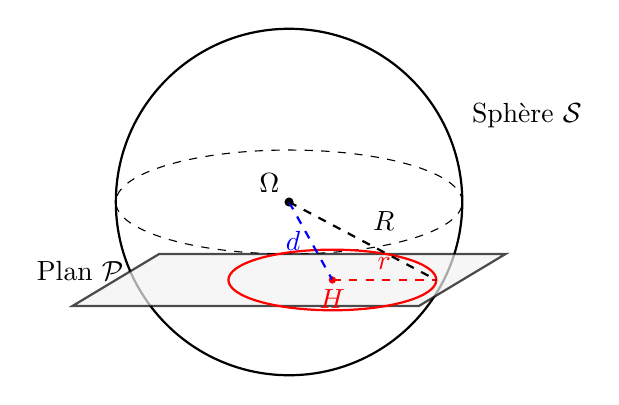
\begin{tikzpicture}[scale=1.1]
  % Dessin de la sphère
  \draw[thick] (0,0) circle (2);
  \draw[dashed] (0,0) ellipse (2 and 0.6);
  \fill (0,0) circle (1.5pt) node[above left] {$\Omega$};
  
  % Dessin du plan sécant (en dessous du centre)
  \draw[thick, fill=gray!10, opacity=0.7] (-2.5, -1.2) -- (1.5, -1.2) -- (2.5, -0.6) -- (-1.5, -0.6) -- cycle;
  
  % Cercle d'intersection
  \draw[red, thick] (0.5, -0.9) ellipse (1.2 and 0.35);
  \fill[red] (0.5, -0.9) circle (1.2pt) node[below] {$H$};
  
  % Ligne de distance et rayon
  \draw[dashed, blue, thick] (0,0) -- (0.5, -0.9) node[midway, left] {$d$};
  \draw[dashed, red, thick] (0.5, -0.9) -- (1.7, -0.9) node[midway, above] {$r$};
  \draw[dashed, black, thick] (0,0) -- (1.7, -0.9) node[midway, above right] {$R$};
  
  \node[right] at (2, 1) {Sphère $\mathcal{S}$};
  \node[left] at (-1.8, -0.8) {Plan $\mathcal{P}$};
\end{tikzpicture}
\end{center}

\subsection{Intersection d'une sphère et d'une droite}

Soit $\mathcal{S}$ une sphère de centre $\Omega$ et de rayon $R$, et $\mathcal{D}$ une droite de représentation paramétrique donnée.
Pour déterminer l'intersection $\mathcal{S} \cap \mathcal{D}$ :
\begin{enumerate}
    \item On injecte les expressions de $x(t)$, $y(t)$ et $z(t)$ de la droite $\mathcal{D}$ dans l'équation cartésienne de la sphère $\mathcal{S}$.
    \item On obtient une équation du second degré d'inconnue $t$.
    \item Selon le signe du discriminant $\Delta$ de cette équation :
    \begin{itemize}
        \item Si $\Delta < 0$ : aucune solution réelle, la droite et la sphère n'ont aucun point d'intersection (la droite passe à l'extérieur).
        \item Si $\Delta = 0$ : une solution réelle unique $t_0$, la droite est tangente à la sphère en un point $H$ de paramètre $t_0$.
        \item Si $\Delta > 0$ : deux solutions réelles $t_1$ et $t_2$, la droite est sécante à la sphère en deux points distincts $M_1$ et $M_2$ de paramètres respectifs $t_1$ et $t_2$.
    \end{itemize}
\end{enumerate}

\section{Méthodes Clés}

\begin{methode}[Déterminer l'équation cartésienne d'un plan]
Pour déterminer l'équation cartésienne d'un plan $\mathcal{P}$ passant par $A(x_A, y_A, z_A)$ et de vecteur normal $\vec{n}(a, b, c)$ :
\begin{enumerate}
    \item L'équation du plan est de la forme $ax + by + cz + d = 0$.
    \item On remplace $x$, $y$ et $z$ par les coordonnées de $A$ pour déterminer la constante $d$ :
    \[
    a x_A + b y_A + c z_A + d = 0 \implies d = -(a x_A + b y_A + c z_A)
    \]
    \item On écrit l'équation finale obtenue.
\end{enumerate}
\end{methode}

\begin{exemple}[Équation de plan]
Soit le plan $\mathcal{P}$ passant par $A(1, -2, 3)$ et de vecteur normal $\vec{n}(2, 1, -1)$.
\begin{enumerate}
    \item Comme $\vec{n}(2, 1, -1)$ est normal à $\mathcal{P}$, l'équation est de la forme : $2x + y - z + d = 0$.
    \item Le point $A(1, -2, 3)$ appartient au plan, donc :
    \[
    2(1) + (-2) - 3 + d = 0 \iff 2 - 2 - 3 + d = 0 \iff d = 3
    \]
    \item L'équation cartésienne du plan $\mathcal{P}$ est donc :
    \[
    2x + y - z + 3 = 0
    \]
\end{enumerate}
\end{exemple}

\section{Exercices d'Entraînement Résolus}

\subsection*{Exercice 1 : Colinéarité de vecteurs et alignement}
Soient les points $A(1, 2, -1)$, $B(3, 0, 5)$ et $C(0, 3, -4)$ dans l'espace muni d'un repère orthonormé. Les points $A$, $B$ et $C$ sont-ils alignés ?

\textbf{Solution :}
Les points $A$, $B$ et $C$ sont alignés si et seulement si les vecteurs $\vec{AB}$ et $\vec{AC}$ sont colinéaires.
Calculons les coordonnées de ces vecteurs :
\[
\vec{AB} = \begin{pmatrix} x_B - x_A \\ y_B - y_A \\ z_B - z_A \end{pmatrix} = \begin{pmatrix} 3 - 1 \\ 0 - 2 \\ 5 - (-1) \end{pmatrix} = \begin{pmatrix} 2 \\ -2 \\ 6 \end{pmatrix}
\]
\[
\vec{AC} = \begin{pmatrix} x_C - x_A \\ y_C - y_A \\ z_C - z_A \end{pmatrix} = \begin{pmatrix} 0 - 1 \\ 3 - 2 \\ -4 - (-1) \end{pmatrix} = \begin{pmatrix} -1 \\ 1 \\ -3 \end{pmatrix}
\]
Cherchons s'il existe un réel $k$ tel que $\vec{AB} = k \vec{AC}$. On remarque immédiatement que :
\[
\vec{AB} = -2 \vec{AC}
\]
En effet, $2 = -2 \times (-1)$, $-2 = -2 \times 1$ et $6 = -2 \times (-3)$.
Les vecteurs $\vec{AB}$ et $\vec{AC}$ sont colinéaires. Par conséquent, les points $A$, $B$ et $C$ sont alignés.

\subsection*{Exercice 2 : Droites parallèles}
Déterminer si la droite $D_1$ passant par le point $A(1, 0, 2)$ et dirigée par le vecteur $\vec{u}_1(2, -1, 3)$ est parallèle à la droite $D_2$ passant par le point $B(0, 3, -1)$ et dirigée par le vecteur $\vec{u}_2(-4, 2, -6)$.

\textbf{Solution :}
Deux droites sont parallèles si et seulement si leurs vecteurs directeurs sont colinéaires.
Comparons les vecteurs directeurs $\vec{u}_1(2, -1, 3)$ et $\vec{u}_2(-4, 2, -6)$ :
On cherche un réel $k$ tel que $\vec{u}_2 = k \vec{u}_1$, ce qui conduit au système :
\[
\begin{cases}
-4 = 2k \\
2 = -k \\
-6 = 3k
\end{cases} \implies k = -2
\]
Le coefficient $k = -2$ convient pour toutes les coordonnées. Les vecteurs $\vec{u}_1$ et $\vec{u}_2$ sont donc colinéaires.
Ainsi, la droite $D_1$ et la droite $D_2$ sont parallèles.

\subsection*{Exercice 3 : Représentation paramétrique de droite}
Soient les points $A(2, -1, 3)$ et $B(0, 4, 1)$.
\begin{enumerate}
    \item Déterminer une représentation paramétrique de la droite $(AB)$.
    \item Le point $C(4, -6, 5)$ appartient-il à cette droite ?
\end{enumerate}

\textbf{Solution :}
\begin{enumerate}
    \item La droite $(AB)$ passe par le point $A(2, -1, 3)$ et a pour vecteur directeur $\vec{AB}$ de coordonnées :
    \[
    \vec{AB} = \begin{pmatrix} 0 - 2 \\ 4 - (-1) \\ 1 - 3 \end{pmatrix} = \begin{pmatrix} -2 \\ 5 \\ -2 \end{pmatrix}
    \]
    Une représentation paramétrique de la droite $(AB)$ est :
    \[
    \begin{cases}
    x = 2 - 2t \\
    y = -1 + 5t \\
    z = 3 - 2t
    \end{cases} \quad (t \in \R)
    \]
    
    \item Le point $C(4, -6, 5)$ appartient à la droite $(AB)$ s'il existe un réel $t$ tel que :
    \[
    \begin{cases}
    4 = 2 - 2t \\
    -6 = -1 + 5t \\
    5 = 3 - 2t
    \end{cases}
    \]
    Résolvons la première équation : $2t = 2 - 4 \implies t = -1$.
    Vérifions si la valeur $t = -1$ satisfait les deux autres équations :
    - Deuxième équation : $-1 + 5(-1) = -6$ (vrai).
    - Troisième équation : $3 - 2(-1) = 5$ (vrai).
    La valeur de paramètre $t = -1$ étant unique et cohérente, le point $C$ appartient à la droite $(AB)$.
\end{enumerate}

\subsection*{Exercice 4 : Coplanarité de vecteurs}
Soient les vecteurs $\vec{u}(1, 2, 0)$, $\vec{v}(0, -1, 3)$ et $\vec{w}(2, 3, 3)$. Les vecteurs $\vec{u}$, $\vec{v}$ et $\vec{w}$ sont-ils coplanaires ?

\textbf{Solution :}
Les vecteurs $\vec{u}$ et $\vec{v}$ ne sont manifestement pas colinéaires (leurs coordonnées ne sont pas proportionnelles).
Les vecteurs $\vec{u}$, $\vec{v}$ et $\vec{w}$ sont coplanaires si et seulement s'il existe deux réels $a$ et $b$ tels que :
\[
\vec{w} = a \vec{u} + b \vec{v}
\]
Ce qui se traduit par le système d'équations :
\[
\begin{cases}
2 = a \times 1 + b \times 0 \\
3 = a \times 2 + b \times (-1) \\
3 = a \times 0 + b \times 3
\end{cases} \iff
\begin{cases}
a = 2 \\
2a - b = 3 \\
3b = 3
\end{cases}
\]
De la première équation, on a $a = 2$.
De la troisième équation, on a $b = 1$.
Injectons ces valeurs dans la deuxième équation pour vérifier la cohérence :
\[
2(2) - (1) = 4 - 1 = 3
\]
La deuxième équation est vérifiée. Le système admet une solution unique $(a, b) = (2, 1)$, donc $\vec{w} = 2\vec{u} + \vec{v}$.
Les vecteurs $\vec{u}$, $\vec{v}$ et $\vec{w}$ sont coplanaires.

\subsection*{Exercice 5 : Orthogonalité et produit scalaire}
Soient les vecteurs $\vec{u}(2, -1, 4)$ et $\vec{v}(3, 2, -1)$ dans un repère orthonormé de l'espace. Calculer le produit scalaire $\vec{u} \cdot \vec{v}$. Les vecteurs $\vec{u}$ et $\vec{v}$ sont-ils orthogonaux ?

\textbf{Solution :}
Le produit scalaire de deux vecteurs dans un repère orthonormé est donné par la formule :
\[
\vec{u} \cdot \vec{v} = x x' + y y' + z z'
\]
Calculons :
\[
\vec{u} \cdot \vec{v} = 2 \times 3 + (-1) \times 2 + 4 \times (-1) = 6 - 2 - 4 = 0
\]
Le produit scalaire étant égal à 0, les vecteurs $\vec{u}$ et $\vec{v}$ sont orthogonaux.

\subsection*{Exercice 6 : Équation cartésienne de plan (Point et Vecteur normal)}
Déterminer une équation cartésienne du plan $\mathcal{P}$ passant par le point $A(1, 3, -2)$ et admettant le vecteur $\vec{n}(2, -1, 5)$ pour vecteur normal.

\textbf{Solution :}
Comme $\vec{n}(2, -1, 5)$ est un vecteur normal au plan $\mathcal{P}$, l'équation cartésienne de $\mathcal{P}$ est de la forme :
\[
2x - y + 5z + d = 0
\]
où $d \in \R$.
Le point $A(1, 3, -2)$ appartient au plan $\mathcal{P}$, ses coordonnées vérifient donc l'équation :
\[
2(1) - (3) + 5(-2) + d = 0 \iff 2 - 3 - 10 + d = 0 \iff -11 + d = 0 \iff d = 11
\]
L'équation cartésienne du plan $\mathcal{P}$ est donc :
\[
2x - y + 5z + 11 = 0
\]

\subsection*{Exercice 7 : Plan défini par trois points}
Soient les points $A(1, 0, 1)$, $B(2, 1, -1)$ et $C(0, 1, 2)$.
\begin{enumerate}
    \item Démontrer que les points $A$, $B$ et $C$ définissent un plan.
    \item Démontrer que le vecteur $\vec{n}(3, 1, 2)$ est un vecteur normal au plan $(ABC)$, puis en déduire une équation cartésienne de ce plan.
\end{enumerate}

\textbf{Solution :}
\begin{enumerate}
    \item Les points $A$, $B$ et $C$ définissent un plan unique si et seulement s'ils ne sont pas alignés, c'est-à-dire si les vecteurs $\vec{AB}$ et $\vec{AC}$ ne sont pas colinéaires.
    Calculons leurs coordonnées :
    \[
    \vec{AB} = \begin{pmatrix} 2-1 \\ 1-0 \\ -1-1 \end{pmatrix} = \begin{pmatrix} 1 \\ 1 \\ -2 \end{pmatrix} \quad \text{et} \quad \vec{AC} = \begin{pmatrix} 0-1 \\ 1-0 \\ 2-1 \end{pmatrix} = \begin{pmatrix} -1 \\ 1 \\ 1 \end{pmatrix}
    \]
    Les coordonnées ne sont pas proportionnelles (par exemple, $\frac{x_{AC}}{x_{AB}} = -1$ et $\frac{y_{AC}}{y_{AB}} = 1$). Les vecteurs ne sont pas colinéaires, donc les points $A, B$ et $C$ définissent bien un plan.
    
    \item Pour prouver que $\vec{n}(3, 1, 2)$ est normal au plan $(ABC)$, il suffit de montrer qu'il est orthogonal aux deux vecteurs directeurs non colinéaires $\vec{AB}$ et $\vec{AC}$ :
    \[
    \vec{n} \cdot \vec{AB} = 3 \times 1 + 1 \times 1 + 2 \times (-2) = 3 + 1 - 4 = 0
    \]
    \[
    \vec{n} \cdot \vec{AC} = 3 \times (-1) + 1 \times 1 + 2 \times 1 = -3 + 1 + 2 = 0
    \]
    Le vecteur $\vec{n}$ est orthogonal à $\vec{AB}$ et $\vec{AC}$, il est donc normal au plan $(ABC)$.
    
    L'équation du plan est de la forme :
    \[
    3x + y + 2z + d = 0
    \]
    Le point $A(1, 0, 1)$ appartient au plan, d'où :
    \[
    3(1) + 0 + 2(1) + d = 0 \iff 5 + d = 0 \iff d = -5
    \]
    L'équation cartésienne du plan $(ABC)$ est :
    \[
    3x + y + 2z - 5 = 0
    \]
\end{enumerate}

\subsection*{Exercice 8 : Intersection droite-plan}
Déterminer l'intersection de la droite $D$ de représentation paramétrique :
\[
\begin{cases}
x = 1 + 2t \\
y = 2 - t \\
z = -1 + 3t
\end{cases} \quad (t \in \R)
\]
et du plan $\mathcal{P}$ d'équation cartésienne $2x + 3y - z - 5 = 0$.

\textbf{Solution :}
Un point $M(x, y, z)$ appartient à l'intersection de la droite $D$ et du plan $\mathcal{P}$ si ses coordonnées vérifient à la fois la représentation paramétrique de $D$ et l'équation de $\mathcal{P}$.
Injectons les expressions de $x$, $y$ et $z$ de la droite dans l'équation cartésienne du plan :
\[
2(1 + 2t) + 3(2 - t) - (-1 + 3t) - 5 = 0
\]
Développons et simplifions :
\[
2 + 4t + 6 - 3t + 1 - 3t - 5 = 0 \iff (4t - 3t - 3t) + (2 + 6 + 1 - 5) = 0 \iff -2t + 4 = 0 \iff t = 2
\]
Il existe une unique valeur de paramètre $t = 2$. La droite et le plan sont donc sécants en un unique point.
Calculons les coordonnées du point d'intersection en remplaçant $t$ par 2 dans la représentation paramétrique de $D$ :
\[
\begin{cases}
x = 1 + 2(2) = 5 \\
y = 2 - (2) = 0 \\
z = -1 + 3(2) = 5
\end{cases}
\]
L'intersection de la droite $D$ et du plan $\mathcal{P}$ est le point $I(5, 0, 5)$.

\subsection*{Exercice 9 : Distance d'un point à un plan par projection}
Soit le plan $\mathcal{P}$ d'équation cartésienne $x - 2y + 2z - 3 = 0$ et le point $A(1, 2, 9)$.
\begin{enumerate}
    \item Déterminer une représentation paramétrique de la droite $D$ orthogonale au plan $\mathcal{P}$ passant par $A$.
    \item Déterminer les coordonnées du projeté orthogonal $H$ du point $A$ sur le plan $\mathcal{P}$.
    \item En déduire la distance $AH$.
\end{enumerate}

\textbf{Solution :}
\begin{enumerate}
    \item Le vecteur normal au plan $\mathcal{P}$ est $\vec{n}(1, -2, 2)$. La droite $D$ étant orthogonale à $\mathcal{P}$, elle admet $\vec{n}$ pour vecteur directeur. Comme elle passe par $A(1, 2, 9)$, sa représentation paramétrique est :
    \[
    \begin{cases}
    x = 1 + t \\
    y = 2 - 2t \\
    z = 9 + 2t
    \end{cases} \quad (t \in \R)
    \]
    
    \item Le projeté orthogonal $H$ de $A$ sur le plan $\mathcal{P}$ est le point d'intersection de la droite $D$ et du plan $\mathcal{P}$. Injectons les équations paramétriques de $D$ dans l'équation de $\mathcal{P}$ :
    \[
    (1 + t) - 2(2 - 2t) + 2(9 + 2t) - 3 = 0 \iff 1 + t - 4 + 4t + 18 + 4t - 3 = 0 \iff 9t + 12 = 0 \iff t = -\frac{4}{3}
    \]
    Remplaçons $t = -\frac{4}{3}$ dans la représentation paramétrique de $D$ pour trouver les coordonnées de $H$ :
    \[
    x_H = 1 - \frac{4}{3} = -\frac{1}{3}, \quad y_H = 2 - 2\left(-\frac{4}{3}\right) = \frac{14}{3}, \quad z_H = 9 + 2\left(-\frac{4}{3}\right) = \frac{19}{3}
    \]
    Le point de projection est $H\left(-\frac{1}{3}, \frac{14}{3}, \frac{19}{3}\right)$.
    
    \item La distance $AH$ is la norme du vecteur $\vec{AH}$. Puisque $H$ est sur la droite $D$, on a $\vec{AH} = t \vec{n}$ avec $t = -\frac{4}{3}$.
    \[
    AH = |t| \times \|\vec{n}\| = \left|-\frac{4}{3}\right| \times \sqrt{1^2 + (-2)^2 + 2^2} = \frac{4}{3} \times \sqrt{1 + 4 + 4} = \frac{4}{3} \times \sqrt{9} = \frac{4}{3} \times 3 = 4
    \]
    La distance du point $A$ au plan $\mathcal{P}$ est de 4 unités.
\end{enumerate}

\subsection*{Exercice 10 : Projeté orthogonal d'un point sur une droite}
Soit la droite $D$ passant par le point $A(1, 1, 1)$ et de vecteur directeur $\vec{u}(2, 1, -1)$. On souhaite déterminer les coordonnées du projeté orthogonal $H$ du point $M(3, 4, 0)$ sur la droite $D$.

\textbf{Solution :}
Puisque $H$ appartient à la droite $D$, il existe un réel $t$ tel que ses coordonnées s'écrivent :
\[
H(1 + 2t, 1 + t, 1 - t)
\]
Le vecteur $\vec{MH}$ a pour coordonnées :
\[
\vec{MH} = \begin{pmatrix} (1 + 2t) - 3 \\ (1 + t) - 4 \\ (1 - t) - 0 \end{pmatrix} = \begin{pmatrix} 2t - 2 \\ t - 3 \\ 1 - t \end{pmatrix}
\]
Par définition, $H$ est le projeté orthogonal de $M$ sur $D$ si et seulement si le vecteur $\vec{MH}$ est orthogonal au vecteur directeur $\vec{u}$ de la droite, soit $\vec{MH} \cdot \vec{u} = 0$ :
\[
2(2t - 2) + 1(t - 3) - 1(1 - t) = 0 \iff 4t - 4 + t - 3 - 1 + t = 0 \iff 6t - 8 = 0 \iff t = \frac{4}{3}
\]
Déterminons les coordonnées de $H$ en remplaçant $t$ par $\frac{4}{3}$ :
\[
x_H = 1 + 2\left(\frac{4}{3}\right) = \frac{11}{3}, \quad y_H = 1 + \frac{4}{3} = \frac{7}{3}, \quad z_H = 1 - \frac{4}{3} = -\frac{1}{3}
\]
Le projeté orthogonal de $M$ sur $D$ est $H\left(\frac{11}{3}, \frac{7}{3}, -\frac{1}{3}\right)$.

\subsection*{Exercice 11 : Calcul de produit vectoriel et aire de triangle}
Soient dans l'espace muni d'un repère orthonormé direct les points $A(1, 2, 0)$, $B(0, 1, 3)$ et $C(2, -1, 1)$.
\begin{enumerate}
    \item Calculer les coordonnées du produit vectoriel $\vec{AB} \wedge \vec{AC}$.
    \item En déduire l'aire du triangle $ABC$.
\end{enumerate}

\textbf{Solution :}
\begin{enumerate}
    \item Déterminons les coordonnées des vecteurs $\vec{AB}$ et $\vec{AC}$ :
    \[
    \vec{AB} = \begin{pmatrix} 0 - 1 \\ 1 - 2 \\ 3 - 0 \end{pmatrix} = \begin{pmatrix} -1 \\ -1 \\ 3 \end{pmatrix} \quad \text{et} \quad \vec{AC} = \begin{pmatrix} 2 - 1 \\ -1 - 2 \\ 1 - 0 \end{pmatrix} = \begin{pmatrix} 1 \\ -3 \\ 1 \end{pmatrix}
    \]
    Calculons le produit vectoriel :
    \[
    \vec{AB} \wedge \vec{AC} = \begin{pmatrix} (-1) \times 1 - 3 \times (-3) \\ 3 \times 1 - (-1) \times 1 \\ (-1) \times (-3) - (-1) \times 1 \end{pmatrix} = \begin{pmatrix} -1 + 9 \\ 3 + 1 \\ 3 + 1 \end{pmatrix} = \begin{pmatrix} 8 \\ 4 \\ 4 \end{pmatrix}
    \]
    
    \item L'aire du triangle $ABC$ est :
    \[
    \mathcal{A}(ABC) = \frac{1}{2} \|\vec{AB} \wedge \vec{AC}\| = \frac{1}{2} \sqrt{8^2 + 4^2 + 4^2} = \frac{1}{2} \sqrt{64 + 16 + 16} = \frac{1}{2} \sqrt{96}
    \]
    Puisque $96 = 16 \times 6$, on a $\sqrt{96} = 4\sqrt{6}$.
    D'où :
    \[
    \mathcal{A}(ABC) = \frac{1}{2} \times 4\sqrt{6} = 2\sqrt{6} \text{ unités d'aire}
    \]
\end{enumerate}

\subsection*{Exercice 12 : Distance d'un point à une droite}
Soit la droite $D$ passant par $A(1, 0, 1)$ et dirigée par le vecteur $\vec{u}(1, 2, -1)$, et soit le point $M(2, 3, 4)$.
Calculer la distance du point $M$ à la droite $D$ en utilisant le produit vectoriel.

\textbf{Solution :}
1. Calculons les coordonnées du vecteur $\vec{AM}$ :
   \[
   \vec{AM} = \begin{pmatrix} 2 - 1 \\ 3 - 0 \\ 4 - 1 \end{pmatrix} = \begin{pmatrix} 1 \\ 3 \\ 3 \end{pmatrix}
   \]
2. Calculons le produit vectoriel $\vec{AM} \wedge \vec{u}$ :
   \[
   \vec{AM} \wedge \vec{u} = \begin{pmatrix} 1 \\ 3 \\ 3 \end{pmatrix} \wedge \begin{pmatrix} 1 \\ 2 \\ -1 \end{pmatrix} = \begin{pmatrix} 3 \times (-1) - 3 \times 2 \\ 3 \times 1 - 1 \times (-1) \\ 1 \times 2 - 3 \times 1 \end{pmatrix} = \begin{pmatrix} -3 - 6 \\ 3 + 1 \\ 2 - 3 \end{pmatrix} = \begin{pmatrix} -9 \\ 4 \\ -1 \end{pmatrix}
   \]
3. Calculons les normes nécessaires :
   - $\|\vec{AM} \wedge \vec{u}\| = \sqrt{(-9)^2 + 4^2 + (-1)^2} = \sqrt{81 + 16 + 1} = \sqrt{98} = 7\sqrt{2}$.
   - $\|\vec{u}\| = \sqrt{1^2 + 2^2 + (-1)^2} = \sqrt{1 + 4 + 1} = \sqrt{6}$.
4. La distance du point $M$ à la droite $D$ est :
   \[
   d(M, D) = \frac{\|\vec{AM} \wedge \vec{u}\|}{\|\vec{u}\|} = \frac{\sqrt{98}}{\sqrt{6}} = \sqrt{\frac{98}{6}} = \sqrt{\frac{49}{3}} = \frac{7}{\sqrt{3}} = \frac{7\sqrt{3}}{3} \text{ unités}
   \]

\subsection*{Exercice 13 : Équation cartésienne d'une sphère}
Dans l'espace muni d'un repère orthonormé, on considère les points $A(2, 1, -3)$ et $B(4, -3, 1)$.
\begin{enumerate}
    \item Déterminer une équation cartésienne de la sphère $\mathcal{S}_1$ de centre $A$ et de rayon $R = 3$.
    \item Déterminer une équation cartésienne de la sphère $\mathcal{S}_2$ de diamètre $[AB]$.
\end{enumerate}

\textbf{Solution :}
\begin{enumerate}
    \item La sphère $\mathcal{S}_1$ a pour centre $A(2, 1, -3)$ et pour rayon $R = 3$. Son équation cartésienne est :
    \[
    (x - 2)^2 + (y - 1)^2 + (z - (-3))^2 = 3^2 \iff (x - 2)^2 + (y - 1)^2 + (z + 3)^2 = 9
    \]
    En développant, on obtient :
    \[
    x^2 - 4x + 4 + y^2 - 2y + 1 + z^2 + 6z + 9 = 9 \iff x^2 + y^2 + z^2 - 4x - 2y + 6z + 5 = 0
    \]
    
    \item Soit $M(x, y, z)$ un point de la sphère $\mathcal{S}_2$ de diamètre $[AB]$. Elle est caractérisée par :
    \[
    \vec{MA} \cdot \vec{MB} = 0 \iff (x - x_A)(x - x_B) + (y - y_A)(y - y_B) + (z - z_A)(z - z_B) = 0
    \]
    Remplaçons par les coordonnées de $A(2, 1, -3)$ et $B(4, -3, 1)$ :
    \[
    (x - 2)(x - 4) + (y - 1)(y + 3) + (z + 3)(z - 1) = 0
    \]
    Développons chaque produit :
    \[
    (x^2 - 6x + 8) + (y^2 + 2y - 3) + (z^2 + 2z - 3) = 0 \iff x^2 + y^2 + z^2 - 6x + 2y + 2z + 2 = 0
    \]
    *Remarque (méthode alternative)* : Le centre $\Omega$ de la sphère est le milieu de $[AB]$, soit $\Omega\left(\frac{2+4}{2}, \frac{1-3}{2}, \frac{-3+1}{2}\right) = \Omega(3, -1, -1)$.
    Le rayon vaut $R = \frac{AB}{2} = \frac{\sqrt{(4-2)^2 + (-3-1)^2 + (1-(-3))^2}}{2} = \frac{\sqrt{4+16+16}}{2} = \frac{\sqrt{36}}{2} = 3$.
    L'équation est $(x - 3)^2 + (y + 1)^2 + (z + 1)^2 = 9 \iff x^2 + y^2 + z^2 - 6x + 2y + 2z + 2 = 0$, ce qui confirme notre résultat.
\end{enumerate}

\subsection*{Exercice 14 : Intersection d'une sphère et d'un plan}
Soit la sphère $\mathcal{S}$ de centre $\Omega(1, -1, 2)$ et de rayon $R = 5$, et soit le plan $\mathcal{P}$ d'équation cartésienne :
\[
2x - y + 2z + 2 = 0
\]
\begin{enumerate}
    \item Calculer la distance $d$ du centre $\Omega$ au plan $\mathcal{P}$.
    \item En déduire que le plan $\mathcal{P}$ coupe la sphère $\mathcal{S}$ selon un cercle $\mathcal{C}$ dont on précisera le rayon $r$.
    \item Déterminer les coordonnées du centre $H$ du cercle $\mathcal{C}$.
\end{enumerate}

\textbf{Solution :}
\begin{enumerate}
    \item La distance du point $\Omega(1, -1, 2)$ au plan $\mathcal{P}$ d'équation $2x - y + 2z + 2 = 0$ est :
    \[
    d = d(\Omega, \mathcal{P}) = \frac{|2x_\Omega - y_\Omega + 2z_\Omega + 2|}{\sqrt{2^2 + (-1)^2 + 2^2}} = \frac{|2(1) - (-1) + 2(2) + 2|}{\sqrt{4 + 1 + 4}} = \frac{|2 + 1 + 4 + 2|}{\sqrt{9}} = \frac{9}{3} = 3
    \]
    
    \item Puisque la distance $d = 3$ est strictement inférieure au rayon $R = 5$, le plan $\mathcal{P}$ coupe la sphère $\mathcal{S}$ selon un cercle $\mathcal{C}$.
    Le rayon $r$ de ce cercle est donné par :
    \[
    r = \sqrt{R^2 - d^2} = \sqrt{5^2 - 3^2} = \sqrt{25 - 9} = \sqrt{16} = 4
    \]
    
    \item Le centre $H$ du cercle $\mathcal{C}$ est le projeté orthogonal de $\Omega$ sur le plan $\mathcal{P}$.
    La droite $\mathcal{D}$ passant par $\Omega(1, -1, 2)$ et orthogonale au plan $\mathcal{P}$ a pour vecteur directeur le vecteur normal au plan $\vec{n}(2, -1, 2)$.
    Une représentation paramétrique de cette droite $\mathcal{D}$ est :
    \[
    \begin{cases}
    x = 1 + 2t \\
    y = -1 - t \\
    z = 2 + 2t
    \end{cases} \quad (t \in \R)
    \]
    Le point $H$ appartient à cette droite et au plan $\mathcal{P}$. Injectons ces coordonnées paramétriques dans l'équation du plan $\mathcal{P}$ :
    \[
    \begin{aligned}
    2(1 + 2t) - (-1 - t) + 2(2 + 2t) + 2 = 0 &\iff 2 + 4t + 1 + t + 4 + 4t + 2 = 0 \\
    &\iff 9t + 9 = 0 \iff t = -1
    \end{aligned}
    \]
    Remplaçons $t = -1$ dans la représentation paramétrique de la droite pour obtenir les coordonnées du centre $H$ :
    \[
    \begin{cases}
    x_H = 1 + 2(-1) = -1 \\
    y_H = -1 - (-1) = 0 \\
    z_H = 2 + 2(-1) = 0
    \end{cases}
    \]
    Le centre du cercle d'intersection est donc $H(-1, 0, 0)$.
\end{enumerate}

\section{Problèmes Résolus}

\subsection*{Problème 1 : Intersection de deux plans et d'une droite}
On se place dans l'espace muni d'un repère orthonormé. On considère les plans $\mathcal{P}_1$ d'équation cartésienne $x - y + z - 2 = 0$ et $\mathcal{P}_2$ d'équation cartésienne $2x + y - z - 1 = 0$.
\begin{enumerate}
    \item Démontrer que les plans $\mathcal{P}_1$ et $\mathcal{P}_2$ se coupent selon une droite $\Delta$.
    \item Déterminer une représentation paramétrique de la droite $\Delta$.
    \item On considère le plan $\mathcal{P}_3$ d'équation cartésienne $x + 2y - z - 3 = 0$. Déterminer l'intersection $\mathcal{P}_1 \cap \mathcal{P}_2 \cap \mathcal{P}_3$.
\end{enumerate}

\textbf{Solution :}
\begin{enumerate}
    \item Les vecteurs normaux respectifs des plans $\mathcal{P}_1$ et $\mathcal{P}_2$ sont $\vec{n}_1(1, -1, 1)$ et $\vec{n}_2(2, 1, -1)$.
    Leurs coordonnées ne sont pas proportionnelles (par exemple, $\frac{2}{1} = 2$ pour l'abscisse mais $\frac{1}{-1} = -1$ pour l'ordonnée). Les vecteurs normaux ne sont pas colinéaires, ce qui signifie que les deux plans ne sont pas parallèles. Ils se coupent donc selon une droite $\Delta$.
    
    \item Un point $M(x, y, z)$ appartient à la droite $\Delta$ si et seulement si ses coordonnées vérifient le système formé par les équations des deux plans :
    \[
    \begin{cases}
    x - y + z - 2 = 0 \quad (1) \\
    2x + y - z - 1 = 0 \quad (2)
    \end{cases}
    \]
    Sommons les équations (1) et (2) membre à membre :
    \[
    (x + 2x) + (-y + y) + (z - z) - 2 - 1 = 0 \iff 3x - 3 = 0 \iff x = 1
    \]
    En remplaçant $x$ par 1 dans l'équation (1) :
    \[
    1 - y + z - 2 = 0 \iff y = z - 1
    \]
    Posons $z = t$ comme paramètre réel ($t \in \R$). On obtient la représentation paramétrique :
    \[
    \begin{cases}
    x = 1 \\
    y = -1 + t \\
    z = t
    \end{cases} \quad (t \in \R)
    \]
    
    \item L'intersection $\mathcal{P}_1 \cap \mathcal{P}_2 \cap \mathcal{P}_3$ est l'intersection de la droite $\Delta = \mathcal{P}_1 \cap \mathcal{P}_2$ avec le plan $\mathcal{P}_3$.
    Injectons les expressions de $x$, $y$ et $z$ de la droite $\Delta$ dans l'équation de $\mathcal{P}_3$ :
    \[
    (1) + 2(-1 + t) - t - 3 = 0 \iff 1 - 2 + 2t - t - 3 = 0 \iff t - 4 = 0 \iff t = 4
    \]
    La valeur du paramètre est $t = 4$. L'intersection est donc un point unique $S$.
    Calculons ses coordonnées :
    \[
    x_S = 1, \quad y_S = -1 + 4 = 3, \quad z_S = 4
    \]
    L'intersection des trois plans est le point $S(1, 3, 4)$.
\end{enumerate}

\subsection*{Problème 2 : Tétraèdre régulier et produit scalaire}
Soit $ABCD$ un tétraèdre régulier d'arête $a > 0$ (toutes ses faces sont des triangles équilatéraux de côté $a$). On note $I$ le milieu du segment $[AB]$ et $J$ le milieu du segment $[CD]$.
\begin{enumerate}
    \item Démontrer que le vecteur $\vec{IJ}$ est orthogonal aux vecteurs $\vec{AB}$ et $\vec{CD}$.
    \item Calculer le produit scalaire $\vec{AB} \cdot \vec{AC}$ en fonction de $a$.
    \item Soit $H$ le projeté orthogonal du point $D$ sur le plan $(ABC)$. Rappeler pourquoi $H$ est le centre de gravité du triangle $ABC$ et exprimer la longueur de la hauteur $DH$ du tétraèdre en fonction de $a$.
\end{enumerate}

\textbf{Solution :}
\begin{enumerate}
    \item Exprimons le vecteur $\vec{IJ}$ en utilisant la relation de Chasles par deux chemins différents :
    \[
    \vec{IJ} = \vec{IA} + \vec{AC} + \vec{CJ}
    \]
    \[
    \vec{IJ} = \vec{IB} + \vec{BD} + \vec{DJ}
    \]
    Sommons ces deux égalités :
    \[
    2\vec{IJ} = (\vec{IA} + \vec{IB}) + (\vec{AC} + \vec{BD}) + (\vec{CJ} + \vec{DJ})
    \]
    Comme $I$ est le milieu de $[AB]$, on a $\vec{IA} + \vec{IB} = \vec{0}$.
    Comme $J$ est le milieu de $[CD]$, on a $\vec{CJ} + \vec{DJ} = \vec{0}$.
    Il reste :
    \[
    2\vec{IJ} = \vec{AC} + \vec{BD} \implies \vec{IJ} = \frac{1}{2}(\vec{AC} + \vec{BD})
    \]
    Calculons le produit scalaire avec $\vec{AB}$ :
    \[
    2\vec{IJ} \cdot \vec{AB} = (\vec{AC} + \vec{BD}) \cdot \vec{AB} = \vec{AC} \cdot \vec{AB} + \vec{BD} \cdot \vec{AB}
    \]
    Les triangles $ABC$ et $ABD$ étant équilatéraux de côté $a$ :
    - $\vec{AC} \cdot \vec{AB} = AC \times AB \times \cos(\frac{\pi}{3}) = a \times a \times \frac{1}{2} = \frac{1}{2}a^2$.
    - $\vec{BD} \cdot \vec{AB} = -\vec{DB} \cdot \vec{AB} = -\vec{BD} \cdot \vec{BA} = -BD \times BA \times \cos(\frac{\pi}{3}) = -a \times a \times \frac{1}{2} = -\frac{1}{2}a^2$.
    Ainsi, $2\vec{IJ} \cdot \vec{AB} = \frac{1}{2}a^2 - \frac{1}{2}a^2 = 0$, donc $\vec{IJ}$ est orthogonal à $\vec{AB}$.
    
    Par symétrie de la configuration géométrique, le même calcul montre que $\vec{IJ}$ est orthogonal à $\vec{CD}$.
    
    \item Le triangle $ABC$ est équilatéral de côté $a$, l'angle en $A$ vaut $60^\circ$ (ou $\frac{\pi}{3}$ radians). Le produit scalaire est :
    \[
    \vec{AB} \cdot \vec{AC} = \|\vec{AB}\| \times \|\vec{AC}\| \times \cos(\widehat{BAC}) = a \times a \times \cos\left(\frac{\pi}{3}\right) = \frac{1}{2}a^2
    \]
    
    \item Par raison de symétrie du tétraèdre régulier, les distances de $D$ aux trois sommets $A$, $B$ et $C$ sont égales. Par conséquent, son projeté orthogonal $H$ sur le plan $(ABC)$ est équidistant de $A$, $B$ et $C$. Dans un triangle équilatéral, le seul point équidistant des trois sommets est son centre de gravité.
    
    Exprimons les longueurs :
    Dans le triangle équilatéral $ABC$ de côté $a$, la longueur d'une médiane (qui est aussi hauteur) est $m = a \frac{\sqrt{3}}{2}$.
    Le centre de gravité $H$ est situé aux deux tiers de chaque médiane en partant du sommet. La distance $AH$ vaut :
    \[
    AH = \frac{2}{3} m = \frac{2}{3} \times a \frac{\sqrt{3}}{2} = \frac{a\sqrt{3}}{3}
    \]
    Le triangle $AHD$ est rectangle en $H$ car $(DH)$ est orthogonale au plan $(ABC)$. D'après le théorème de Pythagore dans ce triangle :
    \[
    AD^2 = AH^2 + DH^2 \iff a^2 = \left(\frac{a\sqrt{3}}{3}\right)^2 + DH^2 \iff a^2 = \frac{3a^2}{9} + DH^2 \iff a^2 = \frac{a^2}{3} + DH^2
    \]
    On en déduit :
    \[
    DH^2 = a^2 - \frac{a^2}{3} = \frac{2}{3}a^2 \implies DH = a \sqrt{\frac{2}{3}} = a\frac{\sqrt{6}}{3}
    \]
    La hauteur d'un tétraèdre régulier de côté $a$ vaut donc $a\frac{\sqrt{6}}{3}$.
\end{enumerate}

\subsection*{Problème 3 : Étude géométrique d'un cube et coordonnées}
Dans l'espace muni d'un repère orthonormé $(O; \vec{\imath}, \vec{\jmath}, \vec{k})$, on considère le cube $OABCDEFG$ de côté 1 tel que $O(0,0,0)$, $A(1,0,0)$, $C(0,1,0)$ et $D(0,0,1)$.
Les sommets restants sont $B(1,1,0)$, $E(1,0,1)$, $F(1,1,1)$ et $G(0,1,1)$.
\begin{enumerate}
    \item Dessiner mentalement le repère. Justifier que $\vec{OF}$ a pour coordonnées $\begin{pmatrix} 1 \\ 1 \\ 1 \end{pmatrix}$.
    \item Soit le plan $(BGE)$. Calculer les coordonnées des vecteurs $\vec{BG}$ et $\vec{BE}$.
    \item Montrer que la grande diagonale $(OF)$ du cube est orthogonale au plan $(BGE)$.
    \item Déterminer une équation cartésienne du plan $(BGE)$.
    \item Soit $H$ le projeté orthogonal de $O$ sur le plan $(BGE)$. Déterminer les coordonnées de $H$ et en déduire la distance de l'origine au plan $(BGE)$.
\end{enumerate}

\textbf{Solution :}
\begin{enumerate}
    \item $O$ est l'origine du repère orthonormé, et $F$ est le sommet opposé du cube. Ses coordonnées sont $F(1, 1, 1)$. Par conséquent, le vecteur diagonal $\vec{OF}$ a pour coordonnées :
    \[
    \vec{OF} = \begin{pmatrix} 1 \\ 1 \\ 1 \end{pmatrix}
    \]
    
    \item Déterminons les coordonnées des vecteurs :
    \[
    \vec{BG} = \begin{pmatrix} x_G-x_B \\ y_G-y_B \\ z_G-z_B \end{pmatrix} = \begin{pmatrix} 0-1 \\ 1-1 \\ 1-0 \end{pmatrix} = \begin{pmatrix} -1 \\ 0 \\ 1 \end{pmatrix}
    \]
    \[
    \vec{BE} = \begin{pmatrix} x_E-x_B \\ y_E-y_B \\ z_E-z_B \end{pmatrix} = \begin{pmatrix} 1-1 \\ 0-1 \\ 1-0 \end{pmatrix} = \begin{pmatrix} 0 \\ -1 \\ 1 \end{pmatrix}
    \]
    
    \item La droite $(OF)$ est orthogonale au plan $(BGE)$ si son vecteur directeur $\vec{OF}$ est orthogonal aux deux vecteurs directeurs non colinéaires $\vec{BG}$ et $\vec{BE}$ du plan. Calculons les produits scalaires :
    \[
    \vec{OF} \cdot \vec{BG} = 1 \times (-1) + 1 \times 0 + 1 \times 1 = -1 + 0 + 1 = 0
    \]
    \[
    \vec{OF} \cdot \vec{BE} = 1 \times 0 + 1 \times (-1) + 1 \times 1 = 0 - 1 + 1 = 0
    \]
    Les produits scalaires étant nuls, le vecteur $\vec{OF}$ est orthogonal à deux vecteurs directeurs sécants du plan. Par conséquent, la droite $(OF)$ est orthogonale au plan $(BGE)$.
    
    \item Puisque $(OF)$ est orthogonale au plan $(BGE)$, le vecteur $\vec{OF}(1, 1, 1)$ est un vecteur normal au plan $(BGE)$. L'équation du plan est donc de la forme :
    \[
    x + y + z + d = 0
    \]
    Le point $B(1, 1, 0)$ appartient à ce plan, ce qui donne :
    \[
    1 + 1 + 0 + d = 0 \iff 2 + d = 0 \iff d = -2
    \]
    Une équation cartésienne du plan $(BGE)$ est :
    \[
    x + y + z - 2 = 0
    \]
    
    \item Le projeté orthogonal $H$ de $O(0,0,0)$ sur le plan $(BGE)$ appartient à la fois au plan et à la droite $(OF)$ passant par $O$ et dirigée par le vecteur normal $\vec{OF}(1,1,1)$.
    La droite $(OF)$ a pour représentation paramétrique $x = t, y = t, z = t$ ($t \in \R$).
    Injectons cela dans l'équation cartésienne du plan :
    \[
    t + t + t - 2 = 0 \iff 3t = 2 \iff t = \frac{2}{3}
    \]
    Les coordonnées de $H$ sont donc $H\left(\frac{2}{3}, \frac{2}{3}, \frac{2}{3}\right)$.
    La distance de l'origine au plan est $OH$ :
    \[
    OH = \sqrt{\left(\frac{2}{3}\right)^2 + \left(\frac{2}{3}\right)^2 + \left(\frac{2}{3}\right)^2} = \sqrt{\frac{4}{9} + \frac{4}{9} + \frac{4}{9}} = \sqrt{\frac{12}{9}} = \frac{\sqrt{12}}{3} = \frac{2\sqrt{3}}{3} \text{ unités}
    \]
\end{enumerate}

\subsection*{Problème 4 : Distance minimale d'un point à une droite et optimisation}
On considère, dans un repère orthonormé de l'espace, la droite $D$ de représentation paramétrique :
\[
\begin{cases}
x = t \\
y = 2t \\
z = 1 - t
\end{cases} \quad (t \in \R)
\]
et deux points fixes $A(1, 1, 1)$ et $B(3, 5, 2)$. On cherche à trouver un point $M$ sur la droite $D$ tel que la somme des carrés des distances de $M$ à $A$ et à $B$ soit minimale.
\begin{enumerate}
    \item Soit $M(t)$ un point de la droite $D$ associé au paramètre $t$. Exprimer $AM^2$ et $BM^2$ en fonction de $t$.
    \item En déduire l'expression de la fonction $f(t) = AM^2 + BM^2$.
    \item Déterminer la valeur $t_0$ pour laquelle la fonction $f$ atteint son minimum.
    \item Donner les coordonnées du point $M_0$ correspondant à ce minimum et calculer la valeur minimale de la fonction $f$.
\end{enumerate}

\textbf{Solution :}
\begin{enumerate}
    \item Les coordonnées de $M$ sont $M(t, 2t, 1-t)$.
    Calculons le carré de la distance $AM$ :
    \[
    \begin{aligned}
    AM^2 &= (t - 1)^2 + (2t - 1)^2 + (1 - t - 1)^2 \\
    &= (t^2 - 2t + 1) + (4t^2 - 4t + 1) + t^2 \\
    &= 6t^2 - 6t + 2
    \end{aligned}
    \]
    Calculons de même le carré de la distance $BM$ :
    \[
    \begin{aligned}
    BM^2 &= (t - 3)^2 + (2t - 5)^2 + (1 - t - 2)^2 \\
    &= (t^2 - 6t + 9) + (4t^2 - 20t + 25) + (-t-1)^2 \\
    &= t^2 - 6t + 9 + 4t^2 - 20t + 25 + t^2 + 2t + 1 \\
    &= 6t^2 - 24t + 35
    \end{aligned}
    \]
    
    \item La somme des carrés s'écrit :
    \[
    f(t) = AM^2 + BM^2 = (6t^2 - 6t + 2) + (6t^2 - 24t + 35) = 12t^2 - 30t + 37
    \]
    
    \item La fonction $f(t)$ est une fonction polynomiale du second degré de la forme $at^2 + bt + c$ avec $a = 12$, $b = -30$ et $c = 37$.
    Comme $a = 12 > 0$, la fonction admet un unique minimum global atteint en :
    \[
    t_0 = -\frac{b}{2a} = -\frac{-30}{2 \times 12} = \frac{30}{24} = \frac{5}{4} = 1,25
    \]
    
    \item Pour $t = 1,25$, les coordonnées du point $M_0$ minimisant la somme sont :
    \[
    x_{M_0} = 1,25, \quad y_{M_0} = 2 \times 1,25 = 2,5, \quad z_{M_0} = 1 - 1,25 = -0,25
    \]
    Le point cherché est $M_0(1,25; 2,5; -0,25)$.
    
    Calculons le minimum de la fonction $f$ :
    \[
    f\left(\frac{5}{4}\right) = 12\left(\frac{5}{4}\right)^2 - 30\left(\frac{5}{4}\right) + 37 = 12 \times \frac{25}{16} - \frac{150}{4} + 37 = \frac{75}{4} - \frac{150}{4} + \frac{148}{4} = \frac{73}{4} = 18,25
    \]
    La somme minimale des carrés des distances est égale à $18,25$.
\end{enumerate}

\subsection*{Problème 5 : Positions relatives et angle formé par deux plans}
On considère les deux plans $\mathcal{P}_1$ d'équation cartésienne $x + y - 2z + 1 = 0$ et $\mathcal{P}_2$ d'équation cartésienne $2x - y + z - 3 = 0$.
\begin{enumerate}
    \item Démontrer que $\mathcal{P}_1$ et $\mathcal{P}_2$ sont sécants et déterminer une représentation paramétrique de leur droite d'intersection $D$.
    \item Calculer le cosinus de l'angle aigu $\theta$ formé par les deux plans (qui correspond à l'angle entre leurs vecteurs normaux).
    \item Soit le point $A(1, 2, 3)$. Calculer la distance du point $A$ au plan $\mathcal{P}_1$ et démontrer que $A$ appartient au plan $\mathcal{P}_2$.
\end{enumerate}

\textbf{Solution :}
\begin{enumerate}
    \item Les vecteurs normaux des plans $\mathcal{P}_1$ et $\mathcal{P}_2$ sont $\vec{n}_1(1, 1, -2)$ et $\vec{n}_2(2, -1, 1)$.
    Leurs coordonnées ne sont pas proportionnelles. Les plans ne sont donc pas parallèles : ils se coupent selon une droite $D$.
    
    Un point $M(x,y,z)$ est sur la droite $D$ si et seulement si ses coordonnées satisfont le système :
    \[
    \begin{cases}
    x + y - 2z + 1 = 0 \quad (1) \\
    2x - y + z - 3 = 0 \quad (2)
    \end{cases}
    \]
    Sommons les deux équations (1) et (2) :
    \[
    3x - z - 2 = 0 \implies z = 3x - 2
    \]
    Remplaçons $z$ par $3x - 2$ dans l'équation (1) :
    \[
    x + y - 2(3x - 2) + 1 = 0 \iff x + y - 6x + 4 + 1 = 0 \iff y = 5x - 5
    \]
    En prenant l'abscisse $x = t$ ($t \in \R$) comme paramètre, on obtient la représentation paramétrique de la droite d'intersection $D$ :
    \[
    \begin{cases}
    x = t \\
    y = -5 + 5t \\
    z = -2 + 3t
    \end{cases} \quad (t \in \R)
    \]
    
    \item Le cosinus de l'angle aigu $\theta$ formé par les deux plans est l'angle aigu formé par leurs vecteurs normaux $\vec{n}_1$ et $\vec{n}_2$. Le produit scalaire est lié à l'angle par la relation :
    \[
    |\vec{n}_1 \cdot \vec{n}_2| = \|\vec{n}_1\| \times \|\vec{n}_2\| \times \cos(\theta) \implies \cos(\theta) = \frac{|\vec{n}_1 \cdot \vec{n}_2|}{\|\vec{n}_1\| \times \|\vec{n}_2\|}
    \]
    Calculons chaque élément :
    - $\vec{n}_1 \cdot \vec{n}_2 = 1 \times 2 + 1 \times (-1) + (-2) \times 1 = 2 - 1 - 2 = -1 \implies |\vec{n}_1 \cdot \vec{n}_2| = 1$.
    - $\|\vec{n}_1\| = \sqrt{1^2 + 1^2 + (-2)^2} = \sqrt{6}$.
    - $\|\vec{n}_2\| = \sqrt{2^2 + (-1)^2 + 1^2} = \sqrt{6}$.
    Par conséquent :
    \[
    \cos(\theta) = \frac{1}{\sqrt{6} \times \sqrt{6}} = \frac{1}{6} \approx 0,167
    \]
    L'angle aigu $\theta$ entre les plans vaut environ $\arccos(1/6) \approx 80,4^\circ$.
    
    \item - La distance du point $A(1, 2, 3)$ au plan $\mathcal{P}_1$ d'équation $x + y - 2z + 1 = 0$ est donnée par la formule :
    \[
    d(A, \mathcal{P}_1) = \frac{|x_A + y_A - 2z_A + 1|}{\sqrt{1^2 + 1^2 + (-2)^2}} = \frac{|1 + 2 - 2(3) + 1|}{\sqrt{6}} = \frac{|4 - 6|}{\sqrt{6}} = \frac{2}{\sqrt{6}} = \frac{\sqrt{6}}{3} \text{ unités}
    \]
    - Injectons les coordonnées de $A(1, 2, 3)$ dans l'équation cartésienne du plan $\mathcal{P}_2$ d'équation $2x - y + z - 3 = 0$ :
    \[
    2(1) - (2) + (3) - 3 = 2 - 2 + 3 - 3 = 0
    \]
    Le résultat étant égal à 0, le point $A$ appartient au plan $\mathcal{P}_2$.
\end{enumerate}
